\documentclass[tikz,border=8pt]{standalone}
\usepackage[T1]{fontenc}
\usepackage{lmodern}
\usepackage{amsmath,amssymb}
\usetikzlibrary{arrows.meta,positioning}
\definecolor{ink}{HTML}{203044}
\definecolor{line}{HTML}{798899}
\definecolor{panel}{HTML}{F4F6F8}
\definecolor{endpoint}{HTML}{EEF5F0}
\begin{document}
\pagecolor{white}
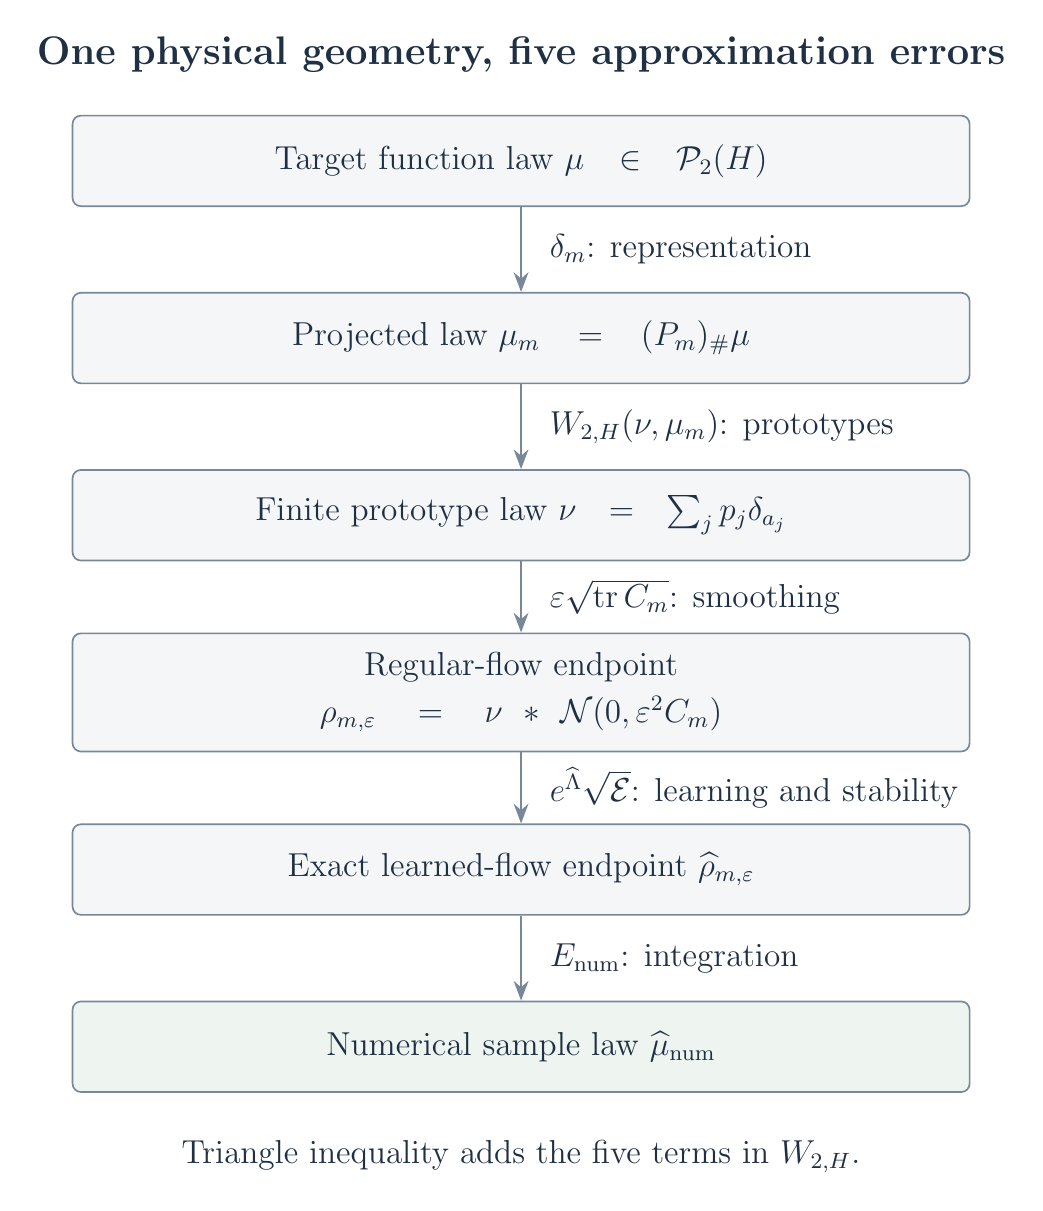
\begin{tikzpicture}[
  text=ink,
  state/.style={draw=line, line width=.6pt, rounded corners=3pt,
    fill=panel, text width=10.9cm, minimum height=1.15cm,
    align=center, inner sep=7pt, font=\large},
  arrow/.style={-{Stealth[length=2.5mm]}, draw=line, line width=.8pt},
  error/.style={font=\large, fill=white, inner sep=4pt, align=left}
]
  \node[font=\Large\bfseries] at (0,1.35) {One physical geometry, five approximation errors};
  \node[state] (target) at (0,0)
    {Target function law \(\mu\in\mathcal P_2(H)\)};
  \node[state] (projected) at (0,-2.25)
    {Projected law \(\mu_m=(P_m)_\#\mu\)};
  \node[state] (prototype) at (0,-4.5)
    {Finite prototype law \(\nu=\sum_jp_j\delta_{a_j}\)};
  \node[state] (smooth) at (0,-6.75)
    {Regular-flow endpoint\\[3pt]
    \(\rho_{m,\varepsilon}=\nu*\mathcal N(0,\varepsilon^2C_m)\)};
  \node[state] (learned) at (0,-9)
    {Exact learned-flow endpoint \(\widehat\rho_{m,\varepsilon}\)};
  \node[state,fill=endpoint] (computed) at (0,-11.25)
    {Numerical sample law \(\widehat\mu_{\rm num}\)};
  \draw[arrow] (target.south) -- (projected.north)
    node[midway,right=6pt,error] {\(\delta_m\): representation};
  \draw[arrow] (projected.south) -- (prototype.north)
    node[midway,right=6pt,error] {\(W_{2,H}(\nu,\mu_m)\): prototypes};
  \draw[arrow] (prototype.south) -- (smooth.north)
    node[midway,right=6pt,error] {\(\varepsilon\sqrt{\operatorname{tr}C_m}\): smoothing};
  \draw[arrow] (smooth.south) -- (learned.north)
    node[midway,right=6pt,error] {\(e^{\widehat\Lambda}\sqrt{\mathcal E}\): learning and stability};
  \draw[arrow] (learned.south) -- (computed.north)
    node[midway,right=6pt,error] {\(E_{\rm num}\): integration};
  \node[font=\large,align=center] at (0,-12.65)
    {Triangle inequality adds the five terms in \(W_{2,H}\).};
\end{tikzpicture}
\end{document}
